\section{Bias}
\dsea is intended to eliminate the bias introduced by the Monte-Carlo-simulated energy spectrum.

In order to test
whether the bias is indeed eliminated,
the model is trained on a \emph{stratified} dataset,
% TODO: explain that dataset: number of events etc.
where each bin contains an equal number of events.
The model is then evaluated on the unmodified dataset.
% TODO: Make clear that train/test data don't overlap
% TODO: This is the opposite of what I did earlier. But it matches what Samuel does. Both should be fine.

The results are shown in \autoref{fig:bias_comparison}.
As can be seen,
only a small bias remains:
The model adapts to the unseen distribution of the test data.
… in comparison to \autoref{fig:bootstrap:spectrum}.

In the work by \citeauthor{dsea_samuel},
relative deviations of more than \SI{1500}{\percent} are observed \cite{dsea_samuel}.
% Aber er schiebt's auf die geringe Accuracy…


\begin{figure}[H]
    \centering
    \begin{subfigure}{0.45\textwidth}
        \centering
        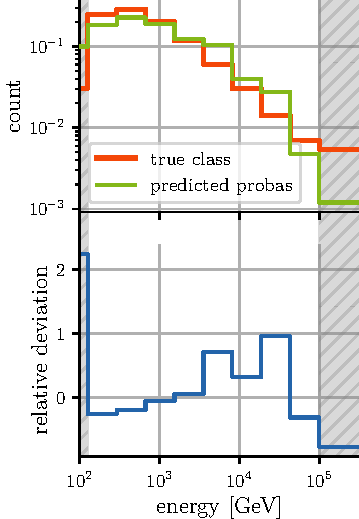
\includegraphics[width=\textwidth]{content/plots/bootstrap:spectrum_half.pdf}
        \caption{
            Placeholder for spectrum A.
            There is bias. Blah.
        }
        % \label{fig:TODO}
    \end{subfigure}
    \begin{subfigure}{0.45\textwidth}
        \centering
        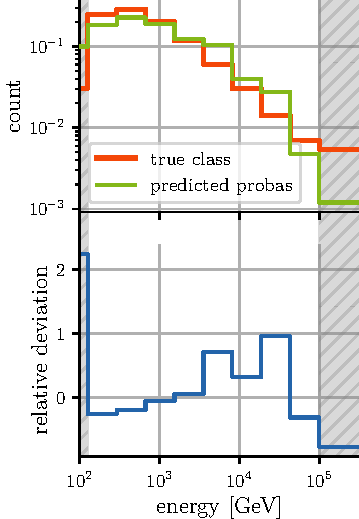
\includegraphics[width=\textwidth]{content/plots/bootstrap:spectrum_half.pdf}
        \caption{
            Placeholder for spectrum B.
            There is no bias. Blah.
        }
        % \label{fig:TODO}
    \end{subfigure}
    \caption{Lorem ipsum dolor sit amet, consectetur adipiscing elit.}
    \label{fig:bias_comparison}
\end{figure}

% TODO: Plot example of a biased reconstruction?
